%-------------------------------------------------------------------------------
% This file provides a skeleton ATLAS note.
% \pdfinclusioncopyfonts=1
% This command may be needed in order to get \ell in PDF plots to appear. Found in
% https://tex.stackexchange.com/questions/322010/pdflatex-glyph-undefined-symbols-disappear-from-included-pdf
%-------------------------------------------------------------------------------
% Specify where ATLAS LaTeX style files can be found.
\newcommand*{\ATLASLATEXPATH}{latex/}
% Use this variant if the files are in a central location, e.g. $HOME/texmf.
% \newcommand*{\ATLASLATEXPATH}{}
%-------------------------------------------------------------------------------
\documentclass[NOTE, atlasdraft=true, texlive=2016, UKenglish]{\ATLASLATEXPATH atlasdoc}
% The language of the document must be set: usually UKenglish or USenglish.
% british and american also work!
% Commonly used options:
%  atlasdraft=true|false This document is an ATLAS draft.
%  texlive=YYYY          Specify TeX Live version (2016 is default).
%  coverpage             Create ATLAS draft cover page for collaboration circulation.
%                        See atlas-draft-cover.tex for a list of variables that should be defined.
%  cernpreprint          Create front page for a CERN preprint.
%                        See atlas-preprint-cover.tex for a list of variables that should be defined.
%  NOTE                  The document is an ATLAS note (draft).
%  PAPER                 The document is an ATLAS paper (draft).
%  CONF                  The document is a CONF note (draft).
%  PUB                   The document is a PUB note (draft).
%  BOOK                  The document is of book form, like an LOI or TDR (draft)
%  txfonts=true|false    Use txfonts rather than the default newtx
%  paper=a4|letter       Set paper size to A4 (default) or letter.

%-------------------------------------------------------------------------------
% Extra packages:
\usepackage[]{\ATLASLATEXPATH atlaspackage}
% Commonly used options:
%  biblatex=true|false   Use biblatex (default) or bibtex for the bibliography.
%  backend=bibtex        Use the bibtex backend rather than biber.
%  subfigure|subfig|subcaption  to use one of these packages for figures in figures.
%  minimal               Minimal set of packages.
%  default               Standard set of packages.
%  full                  Full set of packages.
%-------------------------------------------------------------------------------
% Style file with biblatex options for ATLAS documents.
\usepackage{\ATLASLATEXPATH atlasbiblatex}

% Package for creating list of authors and contributors to the analysis.
\usepackage{\ATLASLATEXPATH atlascontribute}

% Useful macros
\usepackage{\ATLASLATEXPATH atlasphysics}
% See doc/atlas_physics.pdf for a list of the defined symbols.
% Default options are:
%   true:  journal, misc, particle, unit, xref
%   false: BSM, heppparticle, hepprocess, hion, jetetmiss, math, process, other, texmf
% See the package for details on the options.

% Files with references for use with biblatex.
% Note that biber gives an error if it finds empty bib files.
\addbibresource{ANA-HDBS-2020-09-INT1.bib}
\addbibresource{bib/ATLAS.bib}
\addbibresource{bib/CMS.bib}
\addbibresource{bib/ConfNotes.bib}
\addbibresource{bib/PubNotes.bib}
\addbibresource{bib/ATLAS-useful.bib}

% Paths for figures - do not forget the / at the end of the directory name.
\graphicspath{{logos/}{figures/}}

% Add you own definitions here (file ANA-HDBS-2020-09-INT1-defs.sty).
\usepackage{tikz-feynhand}
\usepackage{here}
\usepackage{dcolumn}
\usepackage{scalefnt}
\usepackage{ANA-HDBS-2020-09-INT1-defs}
\usepackage{color}
\usepackage{multirow}
%% \usepackage[hang,small,bf]{caption}
%% \usepackage[subrefformat=parens]{subcaption}
%% \captionsetup{compatibility=false}

%-------------------------------------------------------------------------------
% Generic document information
%-------------------------------------------------------------------------------

% Title, abstract and document
%-------------------------------------------------------------------------------
% This file contains the title, author and abstract.
% It also contains all relevant document numbers used for an ATLAS note.
%-------------------------------------------------------------------------------

% Title
\AtlasTitle{Search for $tb$ resonance using boosted top-quark topology in the lepton+jets final state at $\sqrt{s}=13$ TeV with the ATLAS detector}

% Draft version:
% Should be 1.0 for the first circulation, and 2.0 for the second circulation.
% If given, adds draft version on front page, a 'DRAFT' box on top of each other page, 
% and line numbers.
% Comment or remove in final version.
\AtlasVersion{0.1}

% Abstract - % directly after { is important for correct indentation
\AtlasAbstract{
A search for $tb$ resonances with a boosted top tagging technique is presented, focusing on a final state consisting of a single charged lepton and multiple jets as well as a top-tagged large-$R$ jet. The analysis is based on the pp collision data at the centre-of-mass energy of 13 TeV collected with the ATLAS detector with an integrated luminosity of 139 $\text{fb}^{-1}$. As a hypothetical particle with spin-0(1), a charged Higgs boson (a $W'$ boson) scenario is searched in the mass range from 1 TeV up to 5 TeV.
}

% Author - this does not work with revtex (add it after \begin{document})
% \author{The ATLAS Collaboration}

% Authors and list of contributors to the analysis
% \AtlasAuthorContributor also adds the name to the author list
% Include package latex/atlascontribute to use this
% Use authblk package if there are multiple authors, which is included by latex/atlascontribute
\usepackage{authblk}
% Use the following 3 lines to have all institutes on one line
% \makeatletter
% \renewcommand\AB@affilsepx{, \protect\Affilfont}
% \makeatother
\renewcommand\Authands{, } % avoid ``. and'' for last author
\renewcommand\Affilfont{\itshape\small} % affiliation formatting
\AtlasAuthorContributor{De La Torre Perez, Hector}{a}{W' vs H+ comparisons, W' generation}
\AtlasAuthorContributor{Gombas, Jason Peter}{a}{W' NLO model, W' vs H+ comparisons, W'generation}
\AtlasAuthorContributor{Schwienhorst, Reinhard}{a}{W' NLO model, Jason supervision}
\AtlasAuthorContributor{Sato, Koji}{b}{Analysis contact, supervision of Hiroki}
\AtlasAuthorContributor{Hirose, Shigeki}{b}{Analysis contact, ntuple production, BDT training, MC production, supervision of Hiroki}
\AtlasAuthorContributor{Yamauchi, Hiroki}{b}{Main analyser: ntuple production, fit studies and limits extraction}
\AtlasAuthorContributor{Salvador Salas, Adrian}{c}{Main analyser of resolved analysis, providing technical support; ntuple production}
\AtlasAuthorContributor{Riu, Imma}{c}{Signal AODs and TOPQ1s production; provision of other technical support from resolved analysis}
\AtlasAuthorContributor{Mir Martinez, Lluisa Maria}{c}{Monte Carlo production}
\affil[a]{Michigan State University (US)}
\affil[b]{University of Tsukuba (JP)}
\affil[c]{The Barcelona Institute of Science and Technology (BIST) (ES)}


% \AtlasAuthorContributor{First AtlasAuthorContributor}{a}{Author's contribution.}
% \AtlasAuthorContributor{Second AtlasAuthorContributor}{b}{Author's contribution.}
% \AtlasAuthorContributor{Third AtlasAuthorContributor}{a}{Author's contribution.}
% \AtlasContributor{Fourth AtlasContributor}{Contribution to the analysis.}
%\author[a]{Hiroki Yamaichi}
%\author[a]{Shigeki Hirose}
%\author[b]{Llu\"{i}sa-Maria Mir}
%\author[b]{Imma Riu}
%\author[b]{Adrian Salvador}
%\author[a]{Koji Sato}

%\affil[a]{University of Tsukuba, Japan}
%\affil[b]{Institut de F\'{i}sica d'Altes Energies, Barcelona, Spain}
%\affil[b]{Another Institution}


% If a special author list should be indicated via a link use the following code:
% Include the two lines below if you do not use atlasstyle:
% \usepackage[marginal,hang]{footmisc}
% \setlength{\footnotemargin}{0.5em}
% Use the following lines in all cases:
% \usepackage{authblk}
% \author{The ATLAS Collaboration%
% \thanks{The full author list can be found at:\newline
%   \url{https://atlas.web.cern.ch/Atlas/PUBNOTES/ATL-PHYS-PUB-2016-007/authorlist.pdf}}
% }

% ATLAS reference code, to help ATLAS members to locate the paper
\AtlasRefCode{ANA-HDBS-2020-09}

% ATLAS note number. Can be an COM, INT, PUB or CONF note
\AtlasNote{ANA-HDBS-2020-09-INT1}

% Author and title for the PDF file
\hypersetup{pdftitle={ATLAS document},pdfauthor={The ATLAS Collaboration}}

%-------------------------------------------------------------------------------
% Content
%-------------------------------------------------------------------------------
\begin{document}

\maketitle

\setcounter{tocdepth}{3}
\tableofcontents
\clearpage

% List of contributors - print here or after the Bibliography.
\PrintAtlasContribute{0.30}
\clearpage

%----------------------------------------------------------------------
\textbf{Remaining to do}

\begin{description}

\item[The reweighting method:] A complete proposal is to be discussed at the EB request (HBSM meeting) on 21st July, and incorporate comments and discussions there for the method, summarize them in the note in 1-2 weeks after the meeting.

\item[$W'$ MC production:] Validations are to be finalized by the end of July so that the MC generator can be implemented into the ATLAS official software. We aim for finishing the MC production as well as limit evaluations by the end of September. This is to be done in parallel to EB review, as agreed with the HBSM / HDBS conveners.

\item[Theoretical interpretation: ] Interpret limits in terms of the theoretical H+/W' scenarios, such as hMSSM and XXX. This will be done by the end of September.

\end{description}

\textbf{Version log with major updates:}


\clearpage
%----------------------------------------------------------------------

%---- Section 1
\section{Introduction}
\label{sec:Introduction}

The discovery of a neutral boson with a measured mass around 125 GeV at the Large Hadron Collider (LHC) in 2012 \cite{HIGG-2012-27, CMS-HIG-12-028, HIGG-2014-14} opens the question whether this is the Higgs boson of the Standard Model (SM) or part of an extended scalar sector. Indeed, charged Higgs bosons \footnote{Charge-conjugate is implied elsewhere in this note.} are predicted in several extensions of the SM, which add a second doublet \cite{T.D.Lee-1973, G.Branco-2012, K.Inoue-1982, T.Cheng-1989} or triplets \cite{T.Cheng-1989, J.Schechter-1980, G.Lazarides-1981, R.N.Mohapatra-1981, M.Magg-1980} to its scalar sector. In CP-conserving Two-Higgs-Doublet Models (2HDMs) $H^{+}$ production and decay at tree level depend on its mass and two parameters: the mixing angle $\alpha$ of the neutral CP-even Higgs bosons, and the ratio of the vacuum expectation values of the two Higgs doublets ($\tan{\beta}$).

\begin{figure}[H]
  \centering
  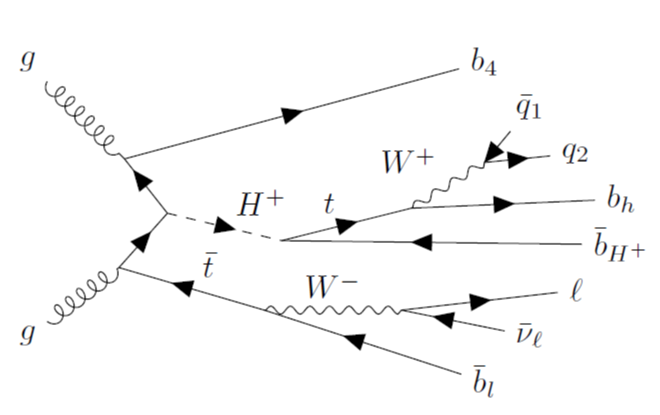
\includegraphics[keepaspectratio,scale=0.5]{images/Introduction/FeynmanDiagram_Htb.png}
  \caption{Feynman diagram for $pp{\rightarrow}tbH^{+}{\rightarrow}tb(tb)$}
  \label{fig:FeynmanDiagram_Htb}
\end{figure}


\vskip.2\baselineskip

For $H^{+}$ masses above the top-quark mass the leading production mode is $gg{\rightarrow}tbH^{+}$ and, close to the alignment limit when $\cos{({\beta}-{\alpha})}{\approx}0$, the dominant decay mode is $H^{+}{\rightarrow}tb$. For lower $H^{+}$ masses, the dominant decay mode is $H^{+}{\rightarrow}{\tau}{\nu}$, as well as for large values of $\tan{\beta}$ irrespective of the charged Higgs mass. Therefore, the two decay modes naturally complement each other in searches for charged Higgs bosons.

\vskip.2\baselineskip

The ATLAS and CMS collaborations have searched for charged Higgs bosons in $pp$ collisions at $\sqrt{s}=7,8$ and 13 TeV, probing the mass range below the top-quark mass in the $\tau\nu$ \cite{HIGG-2012-09, HIGG-2012-22, HIGG-2013-30, CMS-HIG-11-019, CMS-HIG-14-023, HIGG-2016-11}, $cs$ \cite{HIGG-2012-10, CMS-HIG-13-035}, and $cb$ \cite{CMS-HIG-16-030} decay modes, as well as above the top-quark mass in the $\tau\nu$ and $tb$ decay modes \cite{HIGG-2013-30, CMS-HIG-14-023, HIGG-2016-11, HIGG-2013-28, HIGG-2015-11, HIGG-2017-04, HDBS-2021-02, CMS-HIG-18-004, CMS-HIG-18-015, EXOT-2018-32}. In addition, $H^{+}{\rightarrow}WZ$ was searched for in the vector-boson-fusion production mode \cite{HIGG-2014-13, CMS-HIG-16-027}. No evidence for charged Higgs bosons was found in any of these searches.

\vskip.2\baselineskip

This note presents a search for $H^{+}$ production in the $H^{+}{\rightarrow}tb$ decay mode using $pp$ collisions at $\sqrt{s}=13$ TeV. Events with one charged lepton ($l=e,\mu$) and jets in the final state are considered. Compared with the previous analysis using the same final state and the dataset \cite{HDBS-2021-02} (so-called `resolved analysis), boosted top tagging technique is used to identify a hadoronically decaying top quark originated from the decay of the heavy $H^{+}$. This technique allows to improve sensitivities in the high mass regions, where all top decay products are merged into a single large-R jet, and therefore cannot be reconstructed in the resolved analysis \cite{HDBS-2021-02}. 
%Exclusive regions are defined according to the number of jets tagged as originating from the hadronisation of a top quark and $b$-quark.
To separate signal from SM background, multivariate discriminants are employed in the regions where the signal rate is expected to be the largest. Limits on the $H^{+}{\rightarrow}tb$ production cross-section are set by a simultaneous fit of BDT distributions.

\vskip.2\baselineskip

Furthermore, the analysis technique is extended to a search for the $W'{\rightarrow}tb$ decay, where $W'$ is produced in association with $tb$. Several theories beyond the SM predict heavy-charged gauge bosons, which are usually referred to as $W'$ bosons\cite{dienes1999grand,weinberg1979implications,susskind1979dynamics,dimopoulos1979mass,eichten1980dynamical,muller1996topflavor}. Such $W'$ bosons can be heavy enough to decay into a top quark and a bottom quark. Some models predict $W'$ bosons that preferably couple to quarks or third-generation fermions \cite{burdman2006resonances,malkawi1996model,pati1974lepton,hill1995topcolor}. Unlike the $W$ boson, which only couples to left-handed fermions, the chirality of the interaction of the $W'$ boson can be left or right-handed, or a mixture of the two. In models where the right-handed neutrinos are heavier than the right-handed $W'$ boson, such $W'$ bosons cannot be searched for in the leptonic decay modes. We search for $W'$ bosons produced in association with a top quark and a bottom quark, as illustrated in Figure \ref{fig:Wprime_diagram}.

Formerly, $W'$ bosons decaying into a top quark and a bottom quark were searched for in collisions between a quark and an antiquark of any flavour, where the $W'$ boson is singly produced without a top quark.  D0 \cite{abazov2011search} and CDF \cite{aaltonen2009search} Collaborations at the Tevatron and CMS \cite{CMS-EXO-12-001,CMS-B2G-12-010,CMS-B2G-17-010,CMS-B2G-20-005} and ATLAS \cite{TOPQ-2012-19,EXOT-2013-14,EXOT-2017-02,EXOT-2016-18} experiments at the LHC have published such search results.


The analysis replies on ATLAS official background as well as requested $H^+$ and $W'$ signal samples, as detailed in Section~\ref{sec:DataAndMC}, with the TOPQ1 derivation. The ntuples are produced using the TTHbbAnalysis software package.\footnote{https://gitlab.cern.ch/atlasHTop/TTHbbAnalysis/-/tree/user/hyamauch/pflow\_dev\_HplusBoosted} These ntuples are used as inputs to TRExFitter to perform statistical analysis.\footnote{https://gitlab.cern.ch/hyamauch/TRExFitter}

\clearpage
%----------------------------------------------------------------------

%% %----------------------------------------------------------------------
\section{Data and MonteCarlo Simulated Events}
\label{sec:DataAndMC}

\subsection{Data Sample}
\label{subsec:DataSample}
This analysis uses $pp$ collision data collected from 2015 to 2018 by the ATLAS detector at $\sqrt{s}=13$ TeV. Selected events are recorded using unprescaled triggers, as detailed in Table \ref{tab:GlobalLeptonTriggers}. Only runs with stable colliding beams and all ATLAS subsystems operational are used. These are summarized in the Good Run Lists (GRL) shown in Table \ref{tab:GRLForData}, together with the integrated luminosity collected each year. The total integrated luminosity is 139 $\text{fb}^{-1}$ \cite{ATLAS-CONF-2019-021}.

\begin{table}[H]
  \centering
  \subfloat[] {
    \begin{tabular*}{150mm}{@{\extracolsep{\fill}}cc}
      \hline\hline
      Year & Single-electron triggers\\
      \hline
      \multicolumn{1}{l}{2015} & e24\_lhmedium\_L1EM20VH\_OR\_e60\_lhmedium\_OR\_e120\_lhloose\\
      \multicolumn{1}{l}{2016-2018} & e26\_lhtight\_nod0\_ivarloose\_OR\_e60\_lhmedium\_nod0\_OR\_e140\_lhloose\_nod0\\
      \hline\hline
    \end{tabular*}
    \label{tab:SingleElectronTriggers}
  }\\
  \subfloat[] {
    \begin{tabular*}{100mm}{@{\extracolsep{\fill}}cc}
      \hline\hline
      Year & Single-muon triggers\\
      \hline
      \multicolumn{1}{l}{2015} & mu20\_iloose\_L1MU15\_OR\_mu50\\
      \multicolumn{1}{l}{2016-2018} & mu26\_ivarmedium\_OR\_mu50\\
      \hline\hline
    \end{tabular*}
    \label{tab:SingleMuonTriggers}
  }
  \caption{Single-electron (a) and single-muon (b) trigger menus used depending on the year of data-taking.}
  \label{tab:GlobalLeptonTriggers}
\end{table}

\begin{table}[H]
  \centering
  \begin{tabular*}{150mm}{@{\extracolsep{\fill}}ccc}
    \hline\hline
    Year & Luminosity ($\text{pb}^{-1}$) & GRL\\
    \hline
    2015 & 3219.6  & data15\_13TeV/20170619/physics\_25ns\_21.0.19.xml\\
    2016 & 32988.1 & data16\_13TeV/20180129/physics\_25ns\_21.0.19.xml\\
    2017 & 44307.4 & data17\_13TeV/20180619/physics\_25ns\_Triggerno17e33prim.xml\\
    2018 & 58450.1 & data18\_13TeV/20190318/physics\_25ns\_Triggerno17e33prim.xml\\
    \hline\hline
  \end{tabular*}
  \caption{Integrated luminosity for each year of data-taking, computed with the OflLumi-13TeV-010 luminosity
  tag \cite{LuminosityForPhysis}, together with the corresponding GRLs \cite{GoodRunListRun2}.}
  \label{tab:GRLForData}
\end{table}

\subsection{Signal Samples}
\label{subsec:SignalSample}
This paragraph describes MC samples used for each signal event's estimation. The summary is shown in Table \ref{tab:SigSampleSummary}.

\begin{table}[H]
  \centering
  \begin{tabular*}{160mm}{@{\extracolsep{\fill}}lllll}
    \hline\hline
    Physics process & Generator & PS generator & Normalisation & PDF set\\
    \hline
    $tbH^{+}$ ($M_{H^{+}}\leq3.0$ TeV)  & MG5\_aMC 2.6.2 & Pythia 8.212 & NLO & NNPDF2.3NLO\\
    $tbH^{+}$ ($M_{H^{+}}=4.0,5.0$ TeV) & MG5\_aMC 2.8.1 & Pythia 8.244 & NLO & NNPDF3.0NLO\\
    $tbW'$                              & MG5\_aMC 2.9.9 & Pythia 8.307 & NLO & NNPDF3.0NLO\\
    \hline\hline
  \end{tabular*}
  \caption{Nominal simulated signal event samples. The generator, parton shower generator and cross-section used for normalization are shown together with the applied PDF set.}
  \label{tab:SigSampleSummary}
\end{table}

\subsubsection{$\bar{t}bH^{+}$ Samples}
\label{subsec:HpSample}

\newcounter{Num}
\setcounter{Num}{2}

The $H^{+}$ signal samples are generated with MadGraph5\_aMCatNLO (MG5\_aMC) \cite{C.Degrande-2015}, which is a generator based on a four-flavor scheme (4FS) next-to-leading order (NLO) in QCD \cite{Alwall:2014hca}. The NNPDF2.3NLO \cite{Ball:2012cx} parton distribution function (PDF) set is used. \footnote{The samples with masses of 4 and 5 TeV are generated using NNPDF3.0NLO \cite{Ball:2014uwa} PDF set.} The width of the $H^{+}$ is set to zero. Dynamic QCD factorisation and renormalisation scales ($\mu_{f}$ and $\mu_{r}$) are set to $\frac{1}{3}\sum_{i}\sqrt{m(i)^{2}+p_{T}(i)^{2}}$, where $i$ runs over the final state particles ($H^{+}$, $t$ and $b$) used in the generation. The events are showered with Pythia 8.212 \cite{Sjostrand:2007gs} with the A14 \cite{ATL-PHYS-PUB-2014-021} set of underlying-event related parameters tuned to ATLAS. Ten different $H^{+}$ mass points between 1000 and 5000 GeV are generated as detailed in Table \ref{tab:HpSignalSamples}. The table also shows cross sections from MG5\_aMC and Santander-matched cross sections for 2HDM type-\Roman{Num} (a la MSSM), but without SUSY QCD corrections \cite{C.Degrande-2015, M.Flechl-2015, S.Dittmaier-2011, E.L.Berger-2005}. All samples are fully simulated with the proportions of mc16a, mc16d, and mc16e corresponding to the amount of data recorded in the 2015-2016, 2017, and 2018 data-taking years.

\begin{table}[H]
  \centering
  \begin{tabular*}{160mm}{@{\extracolsep{\fill}}cccccc}
    \hline\hline
    DSID   & $H^{+}$ mass [GeV] & Size & ${\sigma}^{\text{MG5\_aMC}}$ [fb] & ${\sigma}_{\tan{\beta}=1}^{\text{MSSM}}$ [fb] & ${\sigma}_{\tan{\beta}=60}^{\text{MSSM}}$ [fb]\\
    \hline
    450004 & 1000 & 1.0M & 3.28                  & 40.9 & 37.8\\
    450598 & 1200 & 1.0M & 1.31                  & 16.4 & 15.1\\
    450599 & 1400 & 1.0M & $5.62{\times}10^{-1}$ &  7.1 &  6.5\\
    450600 & 1600 & 1.2M & $2.54{\times}10^{-1}$ &  3.2 &  3.0\\
    450601 & 1800 & 1.3M & $1.21{\times}10^{-1}$ &  1.5 &  1.4\\
    450602 & 2000 & 1.9M & $5.90{\times}10^{-2}$ &  0.8 &  0.7\\
    451490 & 2500 & 1.9M & $1.11{\times}10^{-2}$ & \multicolumn{2}{c}{\textit{Not available}}\\
    451491 & 3000 & 1.9M & $2.34{\times}10^{-3}$ & \multicolumn{2}{c}{\textit{Not available}}\\     
    508710 & 4000 & 1.9M & $9.75{\times}10^{-5}$ & \multicolumn{2}{c}{\textit{Not available}}\\     
    508711 & 5000 & 1.9M & $4.28{\times}10^{-6}$ & \multicolumn{2}{c}{\textit{Not available}}\\     
    \hline\hline
  \end{tabular*}
  \caption{List of the generated $H^{+}$ samples. All samples are simulated with FullSim and available in the appropriate proportions of mc16a, mc16d, and mc16e. The cross-section values for $\tan{\beta}=1$ or $\tan{\beta}=60$ take into account the production of $H^{\pm}$.}
  \label{tab:HpSignalSamples}
\end{table}

\subsubsection{$\bar{t}bW'$ Samples}
\label{subsec:WpSample}
The left- and right-handed $W'$ ($W'_{L}$ and $W'_{R}$) signal samples are generated with the same options (QCD scales, PDF, NLO, and 4FS) as the $H^{+}$ signal sample generations. Nine different $W'$ mass points between 1000 and 4000 GeV are generated as same as the $H^{+}$ signal samples as detailed in Table \ref{tab:WpSignalSamples} \footnote{Only 5000 GeV mass sample aren't generated, because it is difficult technically due to its very narrow mass width.}. The table also shows cross-sections from MG5\_aMC. All samples are fully simulated with the proportions of mc16a, mc16d, and mc16e corresponding to the amount of data recorded in the 2015-2016, 2017, and 2018 data-taking years. 

\begin{table}[H]
  \centering
  \subfloat[] {
    \begin{tabular*}{130mm}{@{\extracolsep{\fill}}cccc}
        \hline\hline
        DSID   & $W'_{L}$  mass [GeV] & Size & ${\sigma}^{\text{MG5\_aMC}}$ [fb]\\
        \hline
        510889 & 1000                 & 0.5M & 22.54\\
        510890 & 1200                 & 0.5M &  8.56\\
        510891 & 1400                 & 0.5M &  3.50\\
        510892 & 1600                 & 0.5M &  1.53\\
        510893 & 1800                 & 0.5M & $7.03{\times}10^{-1}$ \\
        510894 & 2000                 & 0.5M & $3.33{\times}10^{-1}$ \\
        510895 & 2500                 & 0.5M & $5.98{\times}10^{-2}$ \\
        510896 & 3000                 & 0.5M & $1.19{\times}10^{-2}$ \\     
        510897 & 4000                 & 0.5M & $5.50{\times}10^{-4}$ \\      
        \hline\hline
    \end{tabular*}
    \label{tab:WpLSignalSamples}
  }\\
  \subfloat[] {
    \begin{tabular*}{130mm}{@{\extracolsep{\fill}}cccc}
        \hline\hline
        DSID   & $W'_{R}$ mass [GeV] & Size & ${\sigma}^{\text{MG5\_aMC}}$ [fb]\\
        \hline
        510898 & 1000                & 0.5M & 22.66 \\
        510899 & 1200                & 0.5M &  8.52 \\
        510900 & 1400                & 0.5M &  3.50 \\
        510901 & 1600                & 0.5M &  1.52 \\
        510902 & 1800                & 0.5M & $6.98{\times}10^{-1}$ \\
        510903 & 2000                & 0.5M & $3.33{\times}10^{-1}$ \\
        510904 & 2500                & 0.5M & $5.94{\times}10^{-2}$ \\
        510905 & 3000                & 0.5M & $1.19{\times}10^{-2}$ \\     
        510906 & 4000                & 0.5M & $5.48{\times}10^{-4}$ \\      
        \hline\hline
    \end{tabular*}
    \label{tab:WpRSignalSamples}
  }
  \caption{List of the generated $W'_L$ (a) and $W'_{R}$ (b) samples. All samples are simulated with FullSim and available in the appropriate proportions of mc16a, mc16d, and mc16e.}
  \label{tab:WpSignalSamples}
\end{table}


\subsection{Background Samples}
\label{subsec:BkgSample}
This paragraph describes MC samples used for each background event's estimation. The summary is shown in Table \ref{tab:BkgSampleSummary}.

\begin{table}[H]
  \centering
  \begin{tabular*}{160mm}{@{\extracolsep{\fill}}lllll}
    \hline\hline
    Physics process & Generator & PS generator & Normalisation & PDF set\\
    \hline
    $t\bar{t}+\text{jets}$ & PowhegBox v2   & Pythia 8.230 & NNLO+NNLL & NNPDF3.0NLO\\
    $t\bar{t}H$            & PowhegBox v2   & Pythia 8.230 & NNLO      & NNPDF3.0NLO\\
    $t\bar{t}V$            & MG5\_aMC 2.3.3 & Pythia 8.210 & NLO       & NNPDF3.0NLO\\
    \hline
    Single top t-chan.     & PowhegBox v2   & Pythia 8.230 & aNNLO     & NNPDF3.0NLOnf4\\
    Single top s-chan.     & PowhegBox v2   & Pythia 8.230 & aNNLO     & NNPDF3.0NLO\\
    Single top $tW$        & PowhegBox v2   & Pythia 8.230 & aNNLO     & NNPDF3.0NLO\\
    \hline
    $tHjb$                 & MG5\_aMC 2.6.X & Pythia 8.230 & NLO       & NNPDF3.0NLOnf4\\
    $tHW$                  & MG5\_aMC 2.6.2 & Pythia 8.235 & NLO       & NNPDF3.0NLO\\
    $tZq$                  & MG5\_aMC 2.3.3 & Pythia 8.212 & NLO       & CTEQ6L1LO\\
    $tZW$                  & MG5\_aMC 2.3.3 & Pythia 8.212 & NLO       & NNPDF3.0NLO\\
    4 tops                 & MG5\_aMC 2.3.3 & Pythia 8.230 & NLO       & NNPDF3.1NLO\\
    \hline
    $V+\text{jets}$        & Sherpa 2.2.1   & Sherpa 2.2.1 & NNLO      & NNPDF3.0NLO\\
    Diboson                & Sherpa 2.2     & Sherpa 2.2   & NLO       & NNPDF3.0NLO\\
    \hline\hline
  \end{tabular*}
  \caption{Nominal simulated background event samples. The generator, parton shower generator and cross-section used for normalisation are shown together with the applied PDF set.}
  \label{tab:BkgSampleSummary}
\end{table}


%--- ttbar+jets
\subsubsection{$t\bar{t}$+jets}
\label{subsec:TtbarSamples}
The production of $t\bar{t}$ events is modeled using the PowhegBox \cite{Nason:2004rx, Frixione:2007vw, Alioli:2010xd, J.M.Campbell-2015} v2 generator, which provides matrix element (ME) at NLO in the strong coupling constant ($\alpha_{S}$) with the NNPDF3.0NLO PDF set \cite{Ball:2014uwa} and the $h_{\text{damp}}$ parameter \footnote{The $h_{\text{damp}}$ parameter controls the transverse momentum of the first additional emission beyond the LO Feynman diagram in the parton shower and therefore regulates the high-$p_{\text{T}}$ emission against which the $t\bar{t}$ system recoils.} set to $1.5m_\text{{top}}$ \cite{ATL-PHYS-PUB-2016-020}. The functional form of $\mu_{f}$ and $\mu_{r}$ is set to the default scale $\sqrt{m_{t}^{2}+p_{\text{T},t}^{2}}$. The events are showered with Pythia 8.230 \cite{Sjostrand:2014zea}.

\vskip.2\baselineskip

The uncertainty due to initial-state-radiation (ISR) is estimated using weights in the ME and in the parton shower (PS). To simulate higher parton radiation $\mu_{f}$ and $\mu_{r}$ are varied by a factor of 0.5 in the ME while using the \textit{Var3c} upward variation from the A14 tune. For lower parton radiation, $\mu_{f}$ and $\mu_{r}$ varied by a factor of 2.0 while using the \textit{Var3c} downward variation in the PS. The impact of final-state-radiation (FSR) is evaluated using PS weights which vary $\mu_{r}$ for QCD emission in the FSR by a factor of 0.5 and 2.0, respectively. The impact of the PS and hadronisation model is evaluated by changing the showering of the nominal PowhegBox events from Pythia to Herwig 7.04 \cite{Bahr:2008pv, Bellm:2015jjp}.

\vskip.2\baselineskip

To assess the uncertainty due to the choice of the matching scheme, the Powheg sample is compared to a sample of events generated with MG5\_aMC v2.6.0 and the NNPDF3.0NLO PDF set showered with Pythia 8.230. The shower starting scale has the functional form $\mu_{\text{q}}=H_{\text{T}}/2$ \cite{ATL-PHYS-PUB-2017-007}, where $H_\text{T}$ is defined as the scalar sum of the $p_{\text{T}}$ of all outgoing partons. Choice of $\mu_{f}$ and $\mu_{r}$ is the same as that for the Powheg setup.

\vskip.2\baselineskip

To enhance the statistics in the phase-space relevant for this analysis, for all the samples described above, dedicated filtered samples were produced, requiring $b$- or $c$-hadrons in addition to those arising from the decays of the top quarks, as follows:

\begin{itemize}
  \item One sample was produced with at least two additional $b$-hadrons with $p_{\text{T}}>15$ GeV.
  \item One sample was produced with at least one additional $b$-hadron with $p_{\text{T}}>5$ GeV and failing the previous requirement.
  \item One sample was produced with at least one additional $c$-hadron with $p_{\text{T}}>15$ GeV and failing the previous two requirements.
\end{itemize}

The combined use of the unfiltered and filtered samples is done by assuring no overlap between them (by the use of the heavy flavour filter flag, \textit{TopHeavyFlavorFilterFlag}) and weighted with the appropriate cross-section and filter efficiencies.


%--- ttH
\subsubsection{$t\bar{t}H$}
\label{subsec:TthSamples}

The production of $t\bar{t}H$ events is modeled in the 5F scheme using PowhegBox \cite{Hartanto:2015uka} at NLO in $\alpha_{S}$ with the NNPDF3.0NLO PDF set. The $h_{\text{damp}}$ parameter is set to $3/4\times(m_{t}+m_{\bar{t}}+m_{H})=352.5$ GeV. The events are showered with Pythia 8.230. The uncertainties due to ISR, FSR, PS and hadronisation model, as well as that due to the matching scheme, are evaluated with the same procedures used for the $t\bar{t}+\text{jets}$ background.


%--- ttV
\subsubsection{$t\bar{t}V$}
\label{subsec:TtvSamples}

The production of $t\bar{t}V$ events is modeled using the MG5\_aMC v2.3.3 generator, which provides ME at NLO in $\alpha_{S}$ with the NNPDF3.0NLO PDF set. The functional form of $\mu_{f}$ and $\mu_{r}$ is set to the default scale $0.5{\times}{\sum_{i}}\sqrt{m_{i}^{2}+p_{\text{T},i}^{2}}$ where the sum runs over all the particles generated from the ME calculation. The events are showered with Pythia 8.210.

\vskip.2\baselineskip

Additional $t\bar{t}V$ samples are produced with Sherpa 2.2.0 \cite{Bothmann:2019yzt} at LO accuracy, using the MEPS@LO setup \cite{Catani:2001cc, Hoeche:2009rj} with up to one additional parton for the $t\bar{t}V$ sample and two additional partons for the others. A dynamic $\mu_{r}$ is used, defined similarly to that of the nominal MG5\_aMC+Pythia samples. The CKKW matching scale of the additional emissions is set to 30 GeV. The default Sherpa 2.2.0 PS is used along with the NNPDF3.0NNLO PDF set.


%--- Single top
\subsubsection{Single top}
\label{subsec:SingletopSamples}

\begin{description}
  %--- t-channel
  \item[$t$-channel] \mbox{}\\
    Single-top $t$-channel production is modeled using the PowhegBox v2 generator, which provides ME at NLO in $\alpha_{\text{S}}$ in the 4F scheme with the NNPDF3.0NLOnf4 PDF set. The functional form of $\mu_{f}$ and $\mu_{r}$ is set to $\sqrt{m_{b}^{2}+p_{\text{T},b}^{2}}$, following the recommendation of Ref.~\cite{Frederix:2012dh}. The events are showered with Pythia 8.230.
    \vskip.2\baselineskip
    The impact of the PS and hadronisation model is evaluated by comparing the nominal generator setup with a sample produced with the PowhegBox v2 generator at NLO in QCD in the 4FS using the NNPDF3.0NLOnf4 PDF set. The same events produced for the nominal PowhegBox+Pythia8 sample are used. The events are showered with Herwig 7.04.
    \vskip.2\baselineskip
    To assess the uncertainty due to the choice of the matching scheme, the nominal sample is compared to a sample generated with the MG5\_aMC v2.6.2 generator at NLO in QCD in the 4FS, using the NNPDF3.0NLOnf4 PDF set. Top quarks are decayed at LO using MadSpin \cite{Frixione:2007zp, Artoisenet:2012st} to preserve all spin correlations. The events are showered with Pythia 8.230.
  %--- s-channel    
  \item[$s$-channel] \mbox{}\\
    Single-top $s$-channel production is modeled using the PowhegBox v2 generator, which provides ME at NLO in $\alpha_{\text{S}}$ in the 5F scheme with the NNPDF3.0NLO PDF set. The functional form of $\mu_{f}$ and $\mu_{r}$ is set to the default scale, which is equal to the top quark mass. The events are showered with Pythia 8.230.
    \vskip.2\baselineskip
    The impact of the PS and hadronisation model is evaluated by comparing the nominal generator setup with a sample produced with the PowhegBox v2 generator at NLO in QCD in the 5FSusing the NNPDF3.0NLO PDF set. The same events produced for the nominal PowhegBox+Pythia8 sample are used. The events are showered with Herwig 7.04.
    \vskip.2\baselineskip
    To assess the uncertainty due to choice of the matching scheme, the nominal sample is compared to a sample generated with the MG5\_aMC v2.6.2 generator at NLO in QCD in the 5FS, using the NNPDF3.0NLO PDF set. Top quarks are decayed at LO using MadSpin to preserve all spin correlations. The events are showered with Pythia 8.230.
  %--- tW-channel
  \item[$tW$] \mbox{}\\
    Single-top $tW$ associated production is modeled using the PowhegBox v2 generator, which provides ME at NLO in $\alpha_{\text{S}}$ in the 5F scheme with the NNPDF3.0NLO PDF set. The functional form of $\mu_{f}$ and $\mu_{r}$ is set to the default scale, which is equal to the top quark mass. The diagram removal scheme \cite{Frixione:2008yi} is employed to handle the interference with $t\bar{t}$  production \cite{ATL-PHYS-PUB-2016-020}. The events are showered with Pythia 8.230.
    \vskip.2\baselineskip
    The nominal Powheg+Pythia8 sample is compared to an alternative sample generated using the diagram subtraction scheme \cite{ATL-PHYS-PUB-2016-020, Frixione:2008yi} to estimate the uncertainty due to the interference with $t\bar{t}$ production.
    \vskip.2\baselineskip
    The impact of the PS and hadronisation model is evaluated by comparing the nominal generator setup with a sample produced with the Powheg v2 generator at NLO in QCD in the 5FS using the NNPDF3.0NLO PDF set. The same events produced for the nominal Powheg+Pythia8 sample are used. The events are showered with Herwig7.04.
    \vskip.2\baselineskip
    To assess the uncertainty due to the choice of the matching scheme, the nominal sample is compared to a sample generated with the MG5\_aMC v2.6.2 generator at NLO in QCD in the 5FS, using the NNPDF2.3NLO PDF set. The events are showered with Pythia 8.230.
\end{description}


%--- tH
\subsubsection{$tH$}
\label{subsec:ThSamples}

\begin{description}
  %--- tHjb SM production
  \item[$tHjb$ production] \mbox{}\\
    The production of $tHjb$ events is modeled in the 4F scheme using the MG5\_aMCv2.6.0 with the NNPDF3.0NLOnf4 PDF set. The functional form of $\mu_{f}$ and $\mu_{r}$ is set to the default scale $1/2\times\sum_{i}\sqrt{m_{i}^{2}+p_{\text{T},i}^{2}}$, where the sum runs over all the particles generated from the ME calculation. The shower starting scale has the functional form $\mu_{q}=H_{T}/2$, where $H_{T}$ is defined as the scalar sum of the $p_{\text{T}}$ of all outgoing partons. The events are showered with Pythia 8.230.
  %--- tHW SM production
  \item[$tHW$ production] \mbox{}\\
    The production of $tHW$ events is modeled in the 5F scheme using the MG5\_aMCv2.6.2 with the NNPDF3.0NLO PDF set. The functional form $\mu_{f}$ and $\mu_{r}$ is set to the default scale $1/2\times\sum_{i}\sqrt{m_{i}^{2}+p_{\text{T},i}^{2}}$ where the sum runs over all the particles generated from the ME calculation. The shower starting scale has the functional form $\mu_{q}=H_{T}/2$, where $H_{T}$ is defined as the scalar sum of the $p_{\text{T}}$ of all outgoing partons. The events are showered with Pythia 8.235.
\end{description}


%--- Rare t processes
\subsubsection{Rare $t$ processes}
\label{subsec:RareTopSamples}

\begin{description}
  %--- tZq
  \item[$tZq$] \mbox{}\\
    The $tZq$ MC samples \cite{TOPQ-2016-14} are generated at LO in $\alpha_{\text{S}}$ using MG5\_aMC 2.3.3 in the 4F scheme, with the CTEQ6L1 \cite{Pumplin:2002vw} LO PDF set. Following the recommendations taken from Ref.~\cite{Frederix:2012dh}, the renormalisation and factorisation scales are set to $4\times\sum_{b}\sqrt{m_{i}^{2}+p_{\text{T},b}^{2}}$, where the $b$-quark is the one coming from the gluon splitting. The events are showered with Pythia 8.212.
  %--- tZW
  \item[$tZW$] \mbox{}\\
    The $tZW$ sample is simulated using the MG5\_aMC v2.3.3 generator at NLO in $\alpha_{\text{S}}$ with the NNPDF3.0NLO PDF set. The top quark is decayed inclusively while the $Z$ boson decays to a pair of leptons, by means of Pythia 8.212. The 5F scheme is used where all the quark masses are set to zero, except for the top quark. $\mu_{f}$ and $\mu_{r}$ are set to the top quark mass. The DR1 scheme \cite{Frixione:2008yi} is employed to handle the interference between $tWZ$ and $ttZ$, and is applied to the $tWZ$ sample.
    %--- 4 tops
  \item[4 tops] \mbox{}\\
    The production of 4 tops events is modeled using the MG5\_aMC v2.3.3 generator, which provides ME at NLO in $\alpha_{\text{S}}$ with the NNPDF3.1NLO PDF set. The functional form of $\mu_{f}$ and $\mu_{r}$ is set to $0.25\times\sum_{i}\sqrt{m_{i}^{2}+p_{\text{T},i}^{2}}$, where the sum runs over all the particles generated from the ME calculation, following the Ref.\cite{Frederix:2017wme}. The events are showered with Pythia 8.230.
\end{description}


%--- V+jets
\subsubsection{Vector bosons plus jets}
\label{subsec:VplusJetsSamples}

QCD vector bosons plus jets production is simulated with the Sherpa v2.2.1 PS Monte Carlo generator. In this setup, NLO-accurate ME for up to two jets, and LO-accurate ME for up to four jets are calculated with the Comix \cite{Gleisberg:2008fv} and OpenLoops \cite{Cascioli:2011va, Denner:2016kdg} libraries. The default Sherpa PS \cite{Schumann:2007mg} based on Catani-Seymour dipoles and the cluster hadronisation model \cite{Winter:2003tt} are used. They employ the dedicated set of tuned parameters developed by the Sherpa authors for this version based on the NNPDF3.0nnlo set. The NLO ME of a given jet-multiplicity are matched to the PS using a colour-exact variant of the MC@NLO algorithm \cite{Hoeche:2011fd}. Different jet multiplicities are then merged into an inclusive sample using an improved CKKW matching procedure \cite{Catani:2001cc, Hoeche:2009rj}, which is extended to NLO accuracy using the MEPS@NLO prescription \cite{Hoeche:2012yf}. The merging cut is set to $Q_\text{cut}=20$ GeV.

\vskip.2\baselineskip

QCD scale uncertainties are evaluated on-the-fly \cite{Bothmann:2016nao} using 7-point variations of $\mu_{f}$ and $\mu_{r}$ in the ME. The scales are varied independently by factors of 0.5 and 2 but avoiding opposite factors. PDF uncertainties for the nominal PDF set are evaluated using the 100 variation replicas, as well as $\pm{0.001}$ shifts of $\alpha_{\text{S}}$.


%--- VV
\subsubsection{Dibosons}
\label{subsec:DibosonSamples}

Diboson samples are simulated with the Sherpa v2.2 generator. In this setup multiple ME are matched and merged with the Sherpa PS based on Catani-Seymour dipole using the MEPS@NLO prescription. For semileptonically and fully leptonically decaying diboson samples, as well as loop-induced diboson samples, the virtual QCD correction for ME at NLO accuracy are provided by the OpenLoops library. For electroweak $VVjj$ production, the calculation is performed in the $G_{\mu}$ scheme, ensuring an optimal description of pure electroweak interactions at the electroweak scale. All samples are generated using the NNPDF3.0nnlo set, along with the dedicated set of tuned PS parameters developed by the Sherpa authors.


%% %--- Summary
%% \subsubsection{Summary}
%% \label{subsec:SummarySamples}

%% The samples and their basic generation parameters are summarized in Table \ref{tab:SampleSummary}. Exact dataset names of TOPQ1 DAODs are shown in App. \ref{app:TOPQ1DAODList}

%% \begin{table}[H]
%%   \centering
%%   \begin{tabular*}{160mm}{@{\extracolsep{\fill}}lllll}
%%     \hline\hline
%%     Physics process & Generator & PS generator & Normalisation & PDF set\\
%%     \hline
%%     $tbH^{+}$ ($M_{H^{+}}\leq3.0$ TeV)  & MG5\_aMC 2.6.2 & Pythia 8.212 & NLO & NNPDF2.3NLO\\
%%     $tbH^{+}$ ($M_{H^{+}}=4.0,5.0$ TeV) & MG5\_aMC 2.8.1 & Pythia 8.244 & NLO & NNPDF3.0NLO\\
%%     \hline
%%     $t\bar{t}+\text{jets}$ & PowhegBox v2   & Pythia 8.230 & NNLO+NNLL & NNPDF3.0NLO\\
%%     $t\bar{t}H$            & PowhegBox v2   & Pythia 8.230 & NNLO      & NNPDF3.0NLO\\
%%     $t\bar{t}V$            & MG5\_aMC 2.3.3 & Pythia 8.210 & NLO       & NNPDF3.0NLO\\
%%     \hline
%%     Single top t-chan. & PowhegBox v2 & Pythia 8.230 & aNNLO & NNPDF3.0NLOnf4\\
%%     Single top s-chan. & PowhegBox v2 & Pythia 8.230 & aNNLO & NNPDF3.0NLO\\
%%     Single top $tW$    & PowhegBox v2 & Pythia 8.230 & aNNLO & NNPDF3.0NLO\\
%%     \hline
%%     $tHjb$ & MG5\_aMC 2.6.X & Pythia 8.230 & NLO & NNPDF3.0NLOnf4\\
%%     $tHW$  & MG5\_aMC 2.6.2 & Pythia 8.235 & NLO & NNPDF3.0NLO\\
%%     $tZq$  & MG5\_aMC 2.3.3 & Pythia 8.212 & NLO & CTEQ6L1LO\\
%%     $tZW$  & MG5\_aMC 2.3.3 & Pythia 8.212 & NLO & NNPDF3.0NLO\\
%%     4 tops & MG5\_aMC 2.3.3 & Pythia 8.230 & NLO & NNPDF3.1NLO\\
%%     \hline
%%     $V+\text{jets}$ & Sherpa 2.2.1 & Sherpa 2.2.1 & NNLO & NNPDF3.0NLO\\
%%     Diboson         & Sherpa 2.2   & Sherpa 2.2   & NLO  & NNPDF3.0NLO\\
%%     \hline\hline
%%   \end{tabular*}
%%   \caption{Nominal simulated signal and background event samples. The generator, parton shower generator and cross-section used for normalisation are shown together with the applied PDF set.}
%%   \label{tab:SampleSummary}
%% \end{table}


\clearpage
%% %----------------------------------------------------------------------

% %----------------------------------------------------------------------
% \input{sections/sec3/src/ANA-HDBS-2020-09-INT1-sec3}
% \clearpage
% %----------------------------------------------------------------------

% %----------------------------------------------------------------------
% \input{sections/sec4/src/ANA-HDBS-2020-09-INT1-sec4}
% \clearpage
% %----------------------------------------------------------------------

% %----------------------------------------------------------------------
% \input{sections/sec5/src/ANA-HDBS-2020-09-INT1-sec5}
% \clearpage
% %----------------------------------------------------------------------

% %----------------------------------------------------------------------
% \input{sections/sec6/src/ANA-HDBS-2020-09-INT1-sec6}
% \clearpage
% %----------------------------------------------------------------------

% %----------------------------------------------------------------------
% \input{sections/sec7/src/ANA-HDBS-2020-09-INT1-sec7}
% \clearpage
% %-----------------------------------------------------------------------

% %% %----------------------------------------------------------------------
% %% \input{sections/sec8/src/ANA-HDBS-2020-09-INT1-sec8}
% %% \clearpage
% %% %-----------------------------------------------------------------------

% %% %----------------------------------------------------------------------
% %% \input{sections/sec9/src/ANA-HDBS-2020-09-INT1-sec9}
% %% \clearpage
% %% %-----------------------------------------------------------------------

% %You can find some text snippets that can be used in papers in \texttt{template/atlas-snippets.tex}.
% %Some of the snippets need the \texttt{jetetmiss} option passed to \texttt{atlasphysics}.
% %\input{atlas-snippets}



% %% %-------------------------------------------------------------------------------
% %% \section{Results}
% %% \label{sec:result}
% %% %-------------------------------------------------------------------------------

% %% Place your results here.

% %% % All figures and tables should appear before the summary and conclusion.
% %% % The package placeins provides the macro \FloatBarrier to achieve this.
% %% % \FloatBarrier


% %% %-------------------------------------------------------------------------------
% %% \section{Conclusion}
% %% \label{sec:conclusion}
% %% %-------------------------------------------------------------------------------

% %% Place your conclusion here.


% %-------------------------------------------------------------------------------
% % If you use biblatex and either biber or bibtex to process the bibliography
% % just say \printbibliography here
% \printbibliography
% % If you want to use the traditional BibTeX you need to use the syntax below.
% %\bibliographystyle{bib/bst/atlasBibStyleWithTitle}
% %\bibliography{ANA-HDBS-2020-09-INT1,bib/ATLAS,bib/CMS,bib/ConfNotes,bib/PubNotes}
% %-------------------------------------------------------------------------------

% %-------------------------------------------------------------------------------
% % Print the list of contributors to the analysis
% % The argument gives the fraction of the text width used for the names
% %-------------------------------------------------------------------------------
% %\clearpage
% %% The supporting notes for the analysis should also contain a list of contributors.
% %% This information should usually be included in \texttt{mydocument-metadata.tex}.
% %% The list should be printed either here or before the Table of Contents.
% %% \PrintAtlasContribute{0.30}


% %-------------------------------------------------------------------------------
% \clearpage
% \appendix
% \part*{Appendices}
% \addcontentsline{toc}{part}{Appendices}

% \input{appendices/app1/src/ANA-HDBS-2020-09-INT1-app1}
% \clearpage

% \input{appendices/app2/src/ANA-HDBS-2020-09-INT1-app2}
% \clearpage

% \input{appendices/app3/src/ANA-HDBS-2020-09-INT1-app3}
% \clearpage

% \input{appendices/app4/src/ANA-HDBS-2020-09-INT1-app4}
% \clearpage



%-------------------------------------------------------------------------------
\end{document}
